\documentclass[ProjectRequirements.tex]{subfiles}
\begin{document}

\bigskip

\section{\textsc{\Large Overall Description}}
	\begin{figure}[H]
		\centering
		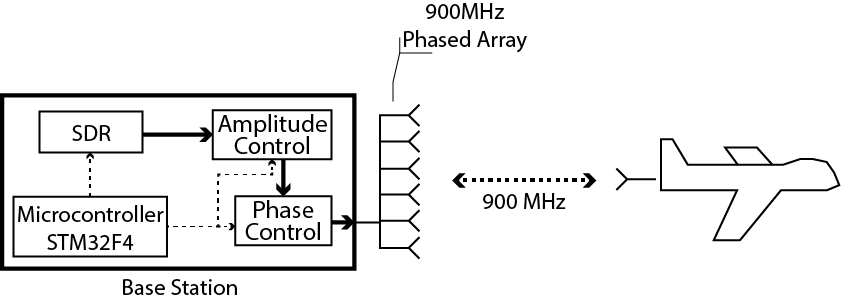
\includegraphics[]{HardwareBlockDiagram.png}
		\caption{Hardware Block Diagram \label{fig:HardwareBlockDiagram}}
	\end{figure}
	\subsection{Product Perspective}
	
		\subsubsection{System Interfaces}
			\begin{itemize}\itemsep1pt
				\item list each one, identify how sw accomplishes the system requirement and the interface description
			\end{itemize}	
		\subsubsection{User Interfaces}
			\begin{itemize}\itemsep1pt
				\item logical characteristics of each interface between the user and the system; required display layouts; forms; reports; constraints due to user characteristics
			\end{itemize}
		\subsubsection{Hardware Interfaces}
			\begin{itemize}\itemsep1pt
				\item \textbf{STM32F4} -- 
				\item \textbf{Xeta SDR} -- 
				\item \textbf{Phased Array} -- \\
				logical characteristics of each interface between the software and the hardware components of the system such as number of ports and their purposes, what devices will be supported for what purpose.
			\end{itemize}
		\subsubsection{Software Interfaces}
			
		
		\subsubsection{Communications Interfaces}
		
		\subsubsection{Memory}
		
		\subsubsection{Operations}
		
	\subsection{Product Functions}
	
		\subsubsection{High Priorities}
		
		\subsubsection{Medium Priorities}
		
		\subsubsection{Low Priorities}
		
	\subsection{User Characteristics}
	
	\subsection{Design Constraints}
	
	\subsection{Assumptions and Dependencies}
	
\end{document}
